\chapter{الوحدات والأبعاد والقياس}\label{ch:b1:units-dimensions}

في مختبرٍ تحت الأرض يتأرجح نواس، وتنقر ساعة إيقاف، ويكتب طالب
$g = \qty{9.77}{m/s^2}$. أهذه هي القيمة ``الصحيحة''؟ يقول الكتاب
$9.81$. أما هل يتفق العددان، وهل صُمِّمت التجربة تصميمًا جيدًا، وأيّ
خطوة من خطواتها هي التي حدّت من دقتها --- فلا شيء من ذلك يُحسم من
الأرقام وحدها. الفيزياء تقيس، وقياسٌ بلا ارتيابه إشاعة. ويضع هذا
الفصل اللغة المشتركة لكل فصل تال: الوحدات والأبعاد ورتب القدر
والحساب الأمين للارتيابات.

\begin{omfigure}
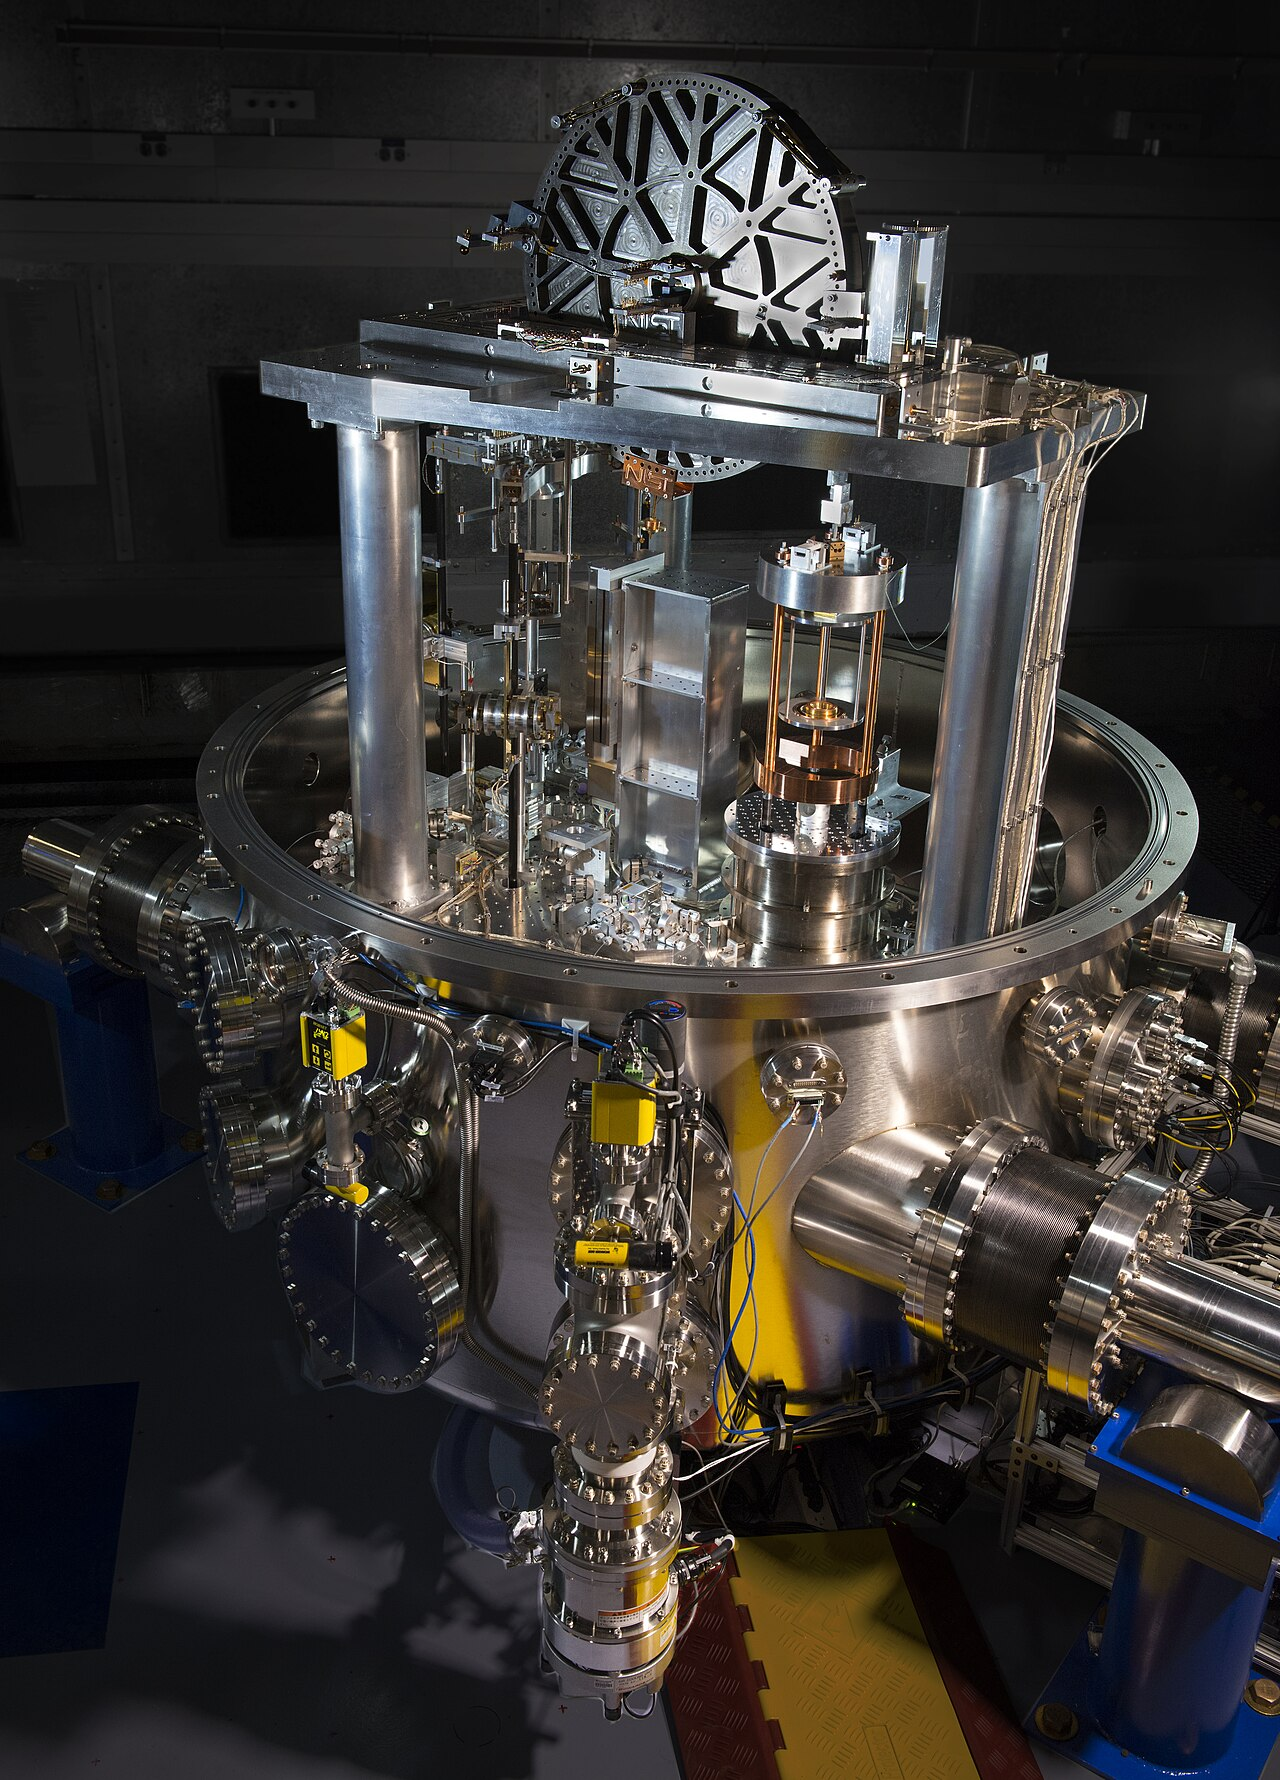
\includegraphics[width=0.46\linewidth]{images/book3/kibble-balance-nist.jpg}

{\small ميزان كِبل NIST من الطراز الرابع، وهو أحد الأجهزة التي تحقق اليوم الكيلوغرام انطلاقًا من ثابت بلانك: تُوزن كتلة في مواجهة قوة كهرمغناطيسية تُقاس بوحدات كهربائية. الصورة: ج. ل. لي، NIST (ملكية عامة).}
\end{omfigure}

\section{النظام الدولي للوحدات}

\begin{definition}[المقدار الفيزيائي والوحدة]\label{def:b1:units-dimensions:unit}
\emph{المقدار الفيزيائي}\index{مقدار فيزيائي} خاصيةٌ يمكن قياسها: طول
أو مدة أو كتلة أو تيار. وقياسه يعني مقارنته بمقدار مرجعي من الجنس
نفسه هو \emph{الوحدة}\index{وحدة}: فالنتيجة عدد مضروب في وحدة،
$\ell = \qty{1.257}{m}$. العدد وحده لا يعني شيئًا، والوحدة وحدها لا
تقيس شيئًا.
\end{definition}

\begin{definition}[الوحدات الأساسية في النظام الدولي]\label{def:b1:units-dimensions:si}
\index{النظام الدولي للوحدات}\index{وحدة أساسية}
يقوم \emph{النظام الدولي للوحدات} (SI) على سبع \emph{وحدات أساسية}:
الثانية (\unit{s}) والمتر (\unit{m}) والكيلوغرام (\unit{kg}) والأمبير
(\unit{A}) والكلفن (\unit{K}) والمول (\unit{mol}) والشمعة (\unit{cd}).
ومنذ 2019 تُعرَّف كل واحدة منها بتثبيت القيمة العددية لثابت من ثوابت
الطبيعة: فالتواتر فوق الدقيق للسيزيوم
$\Delta\nu_{\mathrm{Cs}} = \qty{9192631770}{Hz}$
يعرّف الثانية؛ وسرعة الضوء $c = \qty{299792458}{m/s}$ تعرّف بعدها
المتر؛ وثابت بلانك
$h = \qty{6.62607015e-34}{J.s}$ يعرّف الكيلوغرام؛ والشحنة الأولية
$e = \qty{1.602176634e-19}{C}$ تعرّف الأمبير؛ وثابت بولتزمان
$k_B = \qty{1.380649e-23}{J/K}$ يعرّف الكلفن؛ وثابت أفوغادرو
$N_A = \qty{6.02214076e23}{mol^{-1}}$ يعرّف المول؛ ومردود ضوئي مثبَّت
$K_{\mathrm{cd}}$ يعرّف الشمعة. وكل \omterm{def:b1:units-dimensions:unit}{وحدة} أخرى
\emph{وحدة مشتقة}\index{وحدة مشتقة}، أي جداء قوى لوحدات
أساسية: $\qty{1}{N} = \qty{1}{kg.m/s^2}$، $\qty{1}{J} = \qty{1}{N.m}$،
$\qty{1}{W} = \qty{1}{J/s}$، $\qty{1}{V} = \qty{1}{W/A}$،
$\qty{1}{Pa} = \qty{1}{N/m^2}$.
\end{definition}

\begin{omfigure}
\begin{tikzpicture}[font=\footnotesize, scale=0.95]
  \def\R{3.3} \def\r{1.75}
  \foreach \i/\a/\u/\c in {1/90/{\unit{s}}/{$\Delta\nu_{\mathrm{Cs}}$},
      2/141.4/{\unit{m}}/{$c$}, 3/192.9/{\unit{kg}}/{$h$},
      4/244.3/{\unit{A}}/{$e$}, 5/295.7/{\unit{K}}/{$k_B$},
      6/347.1/{\unit{mol}}/{$N_A$}, 7/38.6/{\unit{cd}}/{$K_{\mathrm{cd}}$}}{
    \node[draw, omDef, thick, circle, minimum size=8.2mm, fill=omDef!8]
      (U\i) at (\a:\R) {\u};
    \node[draw, omThm, circle, minimum size=7.5mm, fill=omThm!6]
      (C\i) at (\a:\r) {\c};
    \draw[-Stealth, omExo] (C\i) -- (U\i);
  }
  \draw[omExo, dashed, -Stealth] (U1) to[bend right=22] (U2);
  \draw[omExo, dashed, -Stealth] (U2) to[bend right=22] (U3);
  \draw[omExo, dashed, -Stealth] (U3) to[bend right=22] (U4);
\end{tikzpicture}

{\small الوحدات الأساسية السبع (الحلقة الخارجية) والثوابت المعرِّفة
السبعة (الحلقة الداخلية). ولا يعرّف ثابتٌ مثبَّت وحدته إلا مع وحدات
سبق تعريفها (بالخط المتقطع): فالثابت $c$ يحوّل الثواني إلى أمتار،
والثابت $h$ يحتاج إلى المتر والثانية لتعريف الكيلوغرام، والشحنة $e$
تحتاج إلى الثانية لتعريف الأمبير.}
\end{omfigure}

\begin{remark}[الأسماء والرموز]\label{rem:b1:units-dimensions:names}
الوحدات المسمّاة بأسماء العلماء تُكتب كاملةً بحروف صغيرة في اللاتينية
(نيوتن، جول، باسكال) ويُرمز إليها بحروف كبيرة (\unit{N}، \unit{J}،
\unit{Pa})؛ فإذا كُتب الاسم كاملًا بحرف أول كبير دلّ على الشخص لا على
\omterm{def:b1:units-dimensions:unit}{الوحدة}. وتتدرج السوابق بقوى العشرة، من p ($10^{-12}$) مرورًا بالسوابق
n و$\mu$ و m و k و M و G وصولًا إلى T ($10^{12}$)؛ والكيلوغرام هو
\omterm{def:b1:units-dimensions:si}{الوحدة الأساسية} الوحيدة التي تحمل سابقة في اسمها.
\end{remark}

\begin{example}[تفكيك وحدة مشتقة]\label{ex:b1:units-dimensions:unpack}
الفولط: $\unit{V} = \unit{W/A} = \unit{J/(A.s)} = \unit{kg.m^2/(A.s^3)}$.
والأوم: $\unit{\ohm} = \unit{V/A} = \unit{kg.m^2/(A^2.s^3)}$. والفاراد:
$\unit{F} = \unit{C/V} = \unit{A.s/V} = \unit{A^2.s^4/(kg.m^2)}$. وهذا
التفكيك أضمن اختبار للتحقق من أن صيغةً حُفظت على وجهها --- ويجعله
القسم التالي منهجيًّا.
\end{example}

\section{التحليل البُعدي}

\begin{definition}[البُعد]\label{def:b1:units-dimensions:dimension}
\index{بُعد}\index{عديم البُعد}
\emph{بُعد} مقدارٍ $X$، ويُكتب $[X]$، يسجّل كيف يُبنى $X$ من المقادير
الأساسية السبعة، بمعزل عن الوحدات المختارة: الطول $L$ والكتلة $M$
والزمن $T$ والتيار الكهربائي $I$ ودرجة الحرارة $\Theta$ وكمية المادة
$N$ وشدة الإضاءة $J$. فللسرعة البعد $[v] = L\,T^{-1}$، وللقوة
$[F] = M\,L\,T^{-2}$، وللطاقة $[E] = M\,L^2\,T^{-2}$. والمقدار الذي
بعده $1$ (زاوية أو نسبة أو قرينة انكسار) \emph{عديم البُعد}.
\end{definition}

\begin{theorem}[مبدأ التجانس البُعدي]\label{thm:b1:units-dimensions:homogeneity}
\index{تجانس بُعدي}
في كل قانون فيزيائي يكون لطرفَي المساواة البعد نفسه، ويكون لكل حدّ من
حدود مجموعٍ بعدُ المجموع كله. أما وسيط الأسّي أو اللوغاريتم أو الجيب
أو جيب التمام فعديم البعد.
\end{theorem}

\begin{proof}
لا تتوقف قوانين الفيزياء على الوحدات التي يختارها الإنسان. وتغيير
\omterm{def:b1:units-dimensions:unit}{وحدة} الطول بعامل $\lambda$ يضرب كل مقدار بعده $L^a \cdots$ في
$\lambda^{-a}$: فمساواةٌ بين حدود مختلفة الأبعاد تصحّ في نظام وحدات
وتفشل في آخر. أما دالة مثل $\exp$ فمتسلسلتها
$1 + x + x^2/2 + \dots$ تجمع قوى $x$ مختلفة الأبعاد ما لم يكن $x$
عديم البعد.
\end{proof}

\begin{method}[التحقق من صيغة]\label{met:b1:units-dimensions:check}
\begin{enumerate}
  \item اكتب \omterm{def:b1:units-dimensions:dimension}{بُعد} كل رمز.
  \item اختزل كل طرف (وكل حدّ) إلى جداء $L^a M^b T^c \cdots$.
  \item إذا تساوت الأسس في الطرفين \emph{جاز} أن تكون الصيغة صحيحة.
        وإذا اختلفت فهي خاطئة قطعًا --- عامل $g$ ساقط، أو مقدار
        مربَّع كان ينبغي أن يبقى بسيطًا، أو أُسّ ذو أبعاد.
\end{enumerate}
وقد تبقى الصيغة المتجانسة خاطئة بعامل عديم البعد ($2$ أو $\pi$ أو
$\tfrac12$): فالأبعاد لا ترى هذه العوامل.
\end{method}

\begin{example}[دور النواس]\label{ex:b1:units-dimensions:pendulum}
نواس طوله $\ell$ وكتلته $m$ يتأرجح في جاذبية $g$. ولنفترض أن دوره
$\tau = k\,\ell^\alpha m^\beta g^\gamma$ حيث $k$ عديم البعد. عندئذٍ
$T = L^\alpha M^\beta (L T^{-2})^\gamma =
L^{\alpha+\gamma} M^\beta T^{-2\gamma}$، ومنه $\beta = 0$ و
$\gamma = -\tfrac12$ و $\alpha = \tfrac12$:
\[
\tau = k\sqrt{\ell/g} .
\]
دون حلّ أي معادلة حركة: تسقط الكتلة، ومضاعفة الطول تضرب الدور في
$\sqrt2$. وستقدّم الديناميك (\cref{ch:b1:oscillators-resonance})
القيمة $k = 2\pi$ للتأرجحات الصغيرة.
\end{example}

\begin{proposition}[التجميعات عديمة البُعد]\label{prop:b1:units-dimensions:pi}
\index{تجميعة عديمة البُعد}
إذا توقف مقدار $Y$ على $n$ من المقادير $X_1, \dots, X_n$ تدخل فيها
$r$ من الأبعاد الأساسية المستقلة، أمكن إعادة كتابة العلاقة بين
$n + 1 - r$ تجميعة عديمة البعد من $X_i$ ومن $Y$. وإذا كان
$n + 1 - r = 1$ وجب أن تكون التجميعة الوحيدة ثابتة، وأعطى التحليل
البعدي القانون إلى حدّ عامل عددي.
\end{proposition}
\admitted

\begin{remark}[استعمال القضية]\label{rem:b1:units-dimensions:pi}
العبارة العامة (مبرهنة فاشي--باكنغهام) قطعة من الجبر الخطي على متجهات
الأسس. والمهم هنا هو الطريقة: أحصِ المقادير ذات الصلة، وعُدّ الأبعاد،
وكوّن التجميعات عديمة البعد. ففي
\cref{ex:b1:units-dimensions:pendulum} لدينا $n = 3$
($\ell, m, g$) و $r = 3$ ($L, M, T$)، فتوجد تجميعة واحدة
$\tau\sqrt{g/\ell}$ ولا بد أن تكون ثابتة. أما قوة السحب على كرة نصف
قطرها $R$ تتحرك بسرعة $v$ في مائع كثافته $\rho$ ولزوجته $\eta$ فتدخل
فيها $n = 4$ مقادير و $r = 3$ أبعاد: أي تجميعتان،
$F/(\rho v^2 R^2)$ و $\rho v R/\eta$ (عدد رينولدز)، ولا تستطيع
الأبعاد وحدها أن تقول كيف تتوقف الأولى على الثانية --- بل التجربة.
\end{remark}

\section{رتب القدر}

\begin{definition}[رتبة القدر]\label{def:b1:units-dimensions:oom}
\index{رتبة القدر}
\emph{رتبة القدر} لمقدارٍ ما هي أقرب قوة من قوى العشرة إليه: فالمقدار
$\qty{6.4e6}{m}$ (نصف قطر الأرض) رتبة قدره $10^7$؛ و$\qty{3e3}{m}$ رتبته
$10^3$؛ و$\qty{3.2e3}{m}$ أقرب إلى $10^3$ منه إلى $10^4$ على سُلّم
لوغاريتمي (والحدّ الفاصل هو $\sqrt{10} \approx 3.16$). ويقال إن
مقدارين ``من الرتبة نفسها'' إذا كانت نسبتهما دون $3$ تقريبًا.
\end{definition}

\begin{method}[التقدير]\label{met:b1:units-dimensions:estimate}
لتقدير مقدار لم يقسه أحد من أجلك:
\begin{enumerate}
  \item فكّكه إلى عوامل تستطيع تقدير كلٍّ منها إلى حدود عامل
        $2$ أو $3$؛
  \item قدّر كل عامل محتفظًا برقم معنوي واحد؛
  \item اضرب محتفظًا بقوة العشرة وبرقم واحد.
\end{enumerate}
تتعاوض أخطاء العوامل المختلفة جزئيًّا، فتكون النتيجة عادةً صحيحة إلى
حدود عامل من $3$ إلى $10$، وهو كل ما يلزم غالبًا لقبول فرضية أو
ردّها.
\end{method}

\begin{example}[كتلة الغلاف الجوي]\label{ex:b1:units-dimensions:atmosphere}
الضغط الجوي $P_0 \approx \qty{1e5}{Pa}$ هو وزن عمود الهواء فوق متر
مربع واحد، $P_0 = m_{\text{عمود}}\,g$، ومنه
$m_{\text{عمود}} \approx 10^5/10 = \qty{1e4}{kg}$ لكل متر مربع.
ومساحة سطح الأرض $4\pi R^2 \approx 4 \times 3 \times (6\times10^6)^2
\approx \qty{5e14}{m^2}$؛ فوزن الغلاف الجوي نحو
$\qty{5e18}{kg}$. والقيمة المعتمدة $\qty{5.1e18}{kg}$ --- ولم يحتج
التقدير إلا إلى $P_0$ و $R$.
\end{example}

\begin{definition}[الأرقام المعنوية]\label{def:b1:units-dimensions:sigfig}
\index{أرقام معنوية}
\emph{الأرقام المعنوية} لعدد مكتوب هي أرقامه ابتداءً من أول رقم غير
معدوم: فللعدد $0.0820$ ثلاثة، وللعدد $\num{8.20e-2}$ الثلاثة نفسها،
أما $820$ فملتبس (رقمان أو ثلاثة) ما لم يُكتب \num{8.2e2} أو
\num{8.20e2}. وتُكتب النتيجة بعدد الأرقام المعنوية التي يسمح بها
ارتيابها (\cref{met:b1:units-dimensions:writing} أدناه): فلا يُكتب
``$g = \qty{9.7723}{m/s^2}$'' والرقم الرابع مجهول.
\end{definition}

\section{ارتياب القياس}

\begin{definition}[المقدار المقيس والخطأ والارتياب]\label{def:b1:units-dimensions:uncertainty}
\index{مقدار مقيس}\index{خطأ القياس}\index{ارتياب معياري}
\emph{المقدار المقيس} هو المقدار الذي يُراد قياسه. وتكرار القياس يعطي
قيمًا متبعثرة: أي إن القياس \emph{متقلّب}. و\emph{خطأ} نتيجةٍ واحدة
هو فرقها المجهول عن القيمة الحقيقية؛ أما \emph{الارتياب المعياري}
$u(x)$ لنتيجة $x$ فهو الانحراف المعياري للقيم التي يمكن أن تُنسب على
نحو معقول إلى المقدار المقيس --- وهو مقدار \emph{يمكن} تقييمه.
ومصادره: المجرِّب (زمن ردّ الفعل، اختلاف المنظر)، والمحيط (درجة
الحرارة، الاهتزازات)، والجهاز (الاستبانة، المعايرة)، والطريقة (نموذج
ليس صحيحًا إلا تقريبًا).
\end{definition}

\begin{proposition}[التقييم من النوع A]\label{prop:b1:units-dimensions:typeA}
\index{ارتياب!النوع A}
من $n$ قيمة مكررة مستقلة $x_1, \dots, x_n$ متوسطها
$\bar x = \frac1n \sum x_i$ وانحرافها المعياري التجريبي
\[
s = \sqrt{\frac{1}{n-1}\sum_{i=1}^n (x_i - \bar x)^2},
\]
يكون أفضل تقدير \omterm{def:b1:units-dimensions:uncertainty}{للمقدار المقيس} هو $\bar x$، ويكون ارتيابه المعياري
\[
u(\bar x) = \frac{s}{\sqrt n} .
\]
\end{proposition}

\begin{proof}[برهان جزئي]
كون $s$ يقدّر تبعثر قياس واحد هو تعريف الانحراف المعياري التجريبي
(بالقسمة على $n - 1$ لا على $n$ لأن المتوسط نفسه قُدّر من المعطيات).
أما كون متوسط $n$ قيمة مستقلة يتبعثر أقلّ $\sqrt n$ مرة من قيمة
واحدة فهو جمع التباينات: تباين مجموع $n$ متغير مستقل يساوي $n$ أضعاف
تباين الواحد، فيكون تباين المتوسط $s^2 n / n^2 = s^2/n$. ودرس
الاحتمالات في هذه السنة يبرهن على العبارتين معًا.
\end{proof}

\begin{omfigure}
\begin{tikzpicture}
\begin{axis}[omaxis, width=9.6cm, height=5.6cm, xlabel={$T$ (\unit{s})},
    ylabel={العدد}, ymin=0, ymax=16, xmin=1.962, xmax=2.058,
    xtick={1.97,1.99,2.01,2.03,2.05},
    x tick label style={/pgf/number format/fixed, /pgf/number format/precision=2}]
  \addplot[ybar, bar width=7.5pt, fill=omDef!35, draw=omDef] coordinates
    {(1.97,1) (1.98,3) (1.99,7) (2.00,12) (2.01,14) (2.02,8) (2.03,4) (2.04,1)};
  \addplot[omThm, thick, domain=1.962:2.058, samples=80] {12.5*exp(-((x-2.009)^2)/(2*0.016^2))};
  \draw[dashed, omExo] (axis cs:2.009,0) -- (axis cs:2.009,15.2) node[above, font=\footnotesize] {$\bar T$};
  \draw[Stealth-Stealth, omExo] (axis cs:1.993,7.6) -- (axis cs:2.025,7.6)
    node[midway, below, font=\footnotesize] {$2s$};
\end{axis}
\end{tikzpicture}

{\small خمسون توقيتًا لدور النواس نفسه، موزَّعة على فئات عرضها
\qty{0.01}{s}. وتبعثرها $s \approx \qty{0.016}{s}$ (لتوقيت واحد)؛
ومتوسط الخمسين معروف إلى $s/\sqrt{50} \approx \qty{0.002}{s}$.
والمنحنى الجرسي غاوسيةٌ لها المتوسط والتبعثر نفسهما.}
\end{omfigure}

\begin{proposition}[التقييم من النوع B]\label{prop:b1:units-dimensions:typeB}
\index{ارتياب!النوع B}
حين تُقرأ قيمة مرة واحدة يُقيَّم ارتيابها ممّا يُعرف عن الجهاز. فإذا
أمكن أن تقع القيمة الحقيقية في أي موضع بين $x - a$ و $x + a$ دون
تفضيل (توزيع \emph{منتظم} نصف عرضه $a$)، كان
\[
u(x) = \frac{a}{\sqrt 3} .
\]
ولسُلّم مدرَّج بخطوة $\delta$ (نصف العرض $a = \delta/2$) يكون
$u = \delta/(2\sqrt3) = \delta/\sqrt{12}$؛ وينطبق الأمر نفسه على آخر
رقم في شاشة رقمية. أما تسامح الصانع المعطى بالصيغة ``$\pm a$''
فيُعالج المعالجة نفسها ما لم تقل بطاقة المعطيات غير ذلك.
\end{proposition}

\begin{proof}
تباين توزيع منتظم على $[x - a, x + a]$ هو
$\frac{1}{2a}\int_{-a}^{a} t^2\,\dd t = \frac{1}{2a}\cdot\frac{2a^3}{3}
= \frac{a^2}{3}$؛ وانحرافه المعياري $a/\sqrt3$.
\end{proof}

\begin{omfigure}
\begin{tikzpicture}[font=\small, x=1.5cm, y=1.6cm]
  \draw[-Stealth] (-0.3,0) -- (4.3,0) node[right] {القيمة};
  \draw[-Stealth] (0,-0.15) -- (0,1.55) node[above] {الكثافة};
  \draw[omDef, very thick] (0.3,0) -- (1.2,0) -- (1.2,1) -- (2.8,1) -- (2.8,0) -- (3.7,0);
  \fill[omDef!20] (1.2,0) rectangle (2.8,1);
  \node[below] at (1.2,0) {$x - a$};
  \node[below] at (2.8,0) {$x + a$};
  \node[below] at (2.0,0) {$x$};
  \node[left] at (0,1) {$\dfrac{1}{2a}$};
  \draw[dashed] (0,1) -- (1.2,1);
  \draw[Stealth-Stealth, omThm, thick] (2.0-0.577*0.8,1.18) -- (2.0+0.577*0.8,1.18)
    node[midway, above] {$2u = 2a/\sqrt3$};
  \draw[dashed, omThm] (2.0,0) -- (2.0,1.18);
\end{tikzpicture}

{\small قراءة لا يُعرف عنها إلا أنها تقع داخل $\pm a$: كثافة منتظمة
$1/(2a)$، وانحراف معياري $a/\sqrt3 \approx 0.58\,a$ --- أصغر من
$a$، لأن الطرفين ليسا أرجح من المركز.}
\end{omfigure}

\begin{theorem}[الارتياب المركّب]\label{thm:b1:units-dimensions:propagation}
\index{ارتياب!مركّب}\index{انتشار الارتيابات}
ليكن $y = f(x_1, \dots, x_n)$ محسوبًا من قيم مقيسة مستقلة ارتياباتها
المعيارية $u(x_i)$. عندئذٍ
\[
u(y)^2 = \sum_{i=1}^n \left(\frac{\partial f}{\partial x_i}\right)^2 u(x_i)^2 .
\]
وبخاصة:
\begin{itemize}
  \item المجموع أو الفرق $y = x_1 \pm x_2$:
        $u(y)^2 = u(x_1)^2 + u(x_2)^2$؛
  \item الجداء أو القسمة $y = x_1 x_2$ أو $x_1/x_2$:
        $\left(\dfrac{u(y)}{y}\right)^2 = \left(\dfrac{u(x_1)}{x_1}\right)^2
        + \left(\dfrac{u(x_2)}{x_2}\right)^2$؛
  \item القوة $y = k\,x^\alpha$: $\dfrac{u(y)}{\abs y} = \abs\alpha\,\dfrac{u(x)}{\abs x}$.
\end{itemize}
\end{theorem}

\begin{proof}
من أجل انحرافات صغيرة $\delta x_i$ يعطي نشر تايلور من الرتبة الأولى
$\delta y = \sum_i (\partial f/\partial x_i)\,\delta x_i$.
والانحرافات مستقلة ومتوسطها معدوم، فتباين المجموع هو مجموع
التباينات، كلٌّ مضروب في مربع معامله --- وهي الصيغة المعروضة. ومنها
تتبع الحالات الخاصة: $\partial(x_1 x_2)/\partial x_1 = x_2$ يعطي
$u(y)^2 = x_2^2 u(x_1)^2 + x_1^2 u(x_2)^2$، ثم نقسم على
$y^2 = x_1^2 x_2^2$؛ ومن أجل $y = kx^\alpha$ يكون
$\partial y/\partial x = \alpha y/x$.
\end{proof}

\begin{example}[كثافة أسطوانة]\label{ex:b1:units-dimensions:density}
أسطوانة: $m = \qty{47.32}{g}$ ($u = \qty{0.01}{g}$)،
$d = \qty{12.00}{mm}$ ($u = \qty{0.02}{mm}$)، $h = \qty{50.2}{mm}$
($u = \qty{0.1}{mm}$). ولدينا $\rho = 4m/(\pi d^2 h)$، فيجمع مربعُ
الارتياب النسبي المقاديرَ $(0.01/47.32)^2 = \num{4.5e-8}$ و
$(2 \times 0.02/12.00)^2 = \num{1.1e-5}$ و
$(0.1/50.2)^2 = \num{4.0e-6}$: فالقطر هو المهيمن، لأنه مربَّع ومقيس
إلى $0.17\%$. ومنه $u(\rho)/\rho = \sqrt{\num{1.5e-5}}
= 0.39\%$؛ و $\rho = \qty{8334}{kg/m^3}$، فيكون
$u(\rho) = \qty{33}{kg/m^3}$: أي
$\rho = (8.33 \pm 0.03)\times10^3\ \unit{kg/m^3}$ --- نحاس أصفر.
\end{example}

\begin{method}[كتابة نتيجة]\label{met:b1:units-dimensions:writing}
\begin{enumerate}
  \item قرّب الارتياب إلى رقم معنوي واحد (أو رقمين إذا كان الأول
        $1$ أو $2$).
  \item قرّب القيمة إلى المرتبة العشرية نفسها.
  \item اكتب القيمة والارتياب مع \omterm{def:b1:units-dimensions:unit}{الوحدة}:
        $g = \qty{9.77\pm0.03}{m/s^2}$، أو $g = \qty{9.77}{m/s^2}$
        مع $u(g) = \qty{0.03}{m/s^2}$.
\end{enumerate}
واحتفظ بأرقام زائدة \emph{أثناء} الحساب، ولا تقرّب إلا في النهاية.
\end{method}

\begin{definition}[الفارق المنسوب]\label{def:b1:units-dimensions:zscore}
\index{فارق منسوب}\index{توافق نتيجتين}
تُقارَن نتيجتان $x_1 \pm u_1$ و $x_2 \pm u_2$ \omterm{def:b1:units-dimensions:uncertainty}{للمقدار المقيس} نفسه
بواسطة \emph{الفارق المنسوب}
\[
z = \frac{\abs{x_1 - x_2}}{\sqrt{u_1^2 + u_2^2}} .
\]
وتكونان \emph{متوافقتين} إذا كان $z \leq 2$؛ أما $z$ الأكبر فيشير
إلى أثر لم يُحسب حسابه --- أو إلى ارتياب مقدَّر بأقلّ من قيمته. وإذا
كان $x_2$ قيمة مرجعية بلا ارتياب معلن أُخذ $u_2 = 0$.
\end{definition}

\begin{remark}[لماذا 2]\label{rem:b1:units-dimensions:why2}
إذا تبعثرت النتيجتان تبعثرًا غاوسيًّا كان لفرقهما انحراف معياري
$\sqrt{u_1^2 + u_2^2}$، والغاوسية تتجاوز ضعف انحرافها المعياري في نحو
$5\%$ من الحالات. والشرط ``$z \leq 2$'' اصطلاح لا مبرهنة: فهو يعدّ
نحو قياس جيد واحد من كل عشرين اختلافًا زائفًا.
\end{remark}

\section{ملاءمة نموذج للمعطيات}

\begin{proposition}[مستقيم المربعات الصغرى]\label{prop:b1:units-dimensions:regression}
\index{انحدار خطي}\index{المربعات الصغرى}
لتكن $n$ نقطة $(x_i, y_i)$ يُنتظر أن تخضع للعلاقة $y = a x + b$؛
فالمستقيم الذي يصغّر مجموع مربعات المسافات الشاقولية
$\sum_i (y_i - a x_i - b)^2$ له
\[
a = \frac{\sum_i (x_i - \bar x)(y_i - \bar y)}{\sum_i (x_i - \bar x)^2},
\qquad
b = \bar y - a\,\bar x .
\]
\end{proposition}

\begin{proof}
المجموع دالة من الدرجة الثانية في $(a, b)$؛ وبمساواة المشتقين
الجزئيين بالصفر نحصل على معادلتين خطيتين:
$\sum_i (y_i - ax_i - b) = 0$، أي $\bar y = a \bar x + b$، و
$\sum_i x_i (y_i - ax_i - b) = 0$. وبتعويض $b$ في الثانية وتوسيط
المتغيرات نجد $a$. أما التصغير نفسه فيُجرى في درس الرياضيات حول دوال
متغيرين.
\end{proof}

\begin{method}[التحقق البياني من نموذج]\label{met:b1:units-dimensions:fit}
\begin{enumerate}
  \item اختر متغيرات تجعل القانون المنتظر مستقيمًا:
        $\tau^2$ بدلالة $\ell$ للنواس، و$\ln y$ بدلالة
        $\ln x$ لقانون قوة $y = Cx^\alpha$ (الميل $\alpha$).
  \item ارسم النقاط \emph{مع قضبان ارتيابها}.
  \item لائم المستقيم؛ ويكون النموذج مقبولًا إذا تخطّت القضبان
        المستقيم دون نزعة منتظمة في البواقي، وإذا كان المقطع هو ما
        يتنبأ به النموذج (وهو الصفر هنا).
  \item اقرأ الفيزياء من الميل، مع ارتيابه.
\end{enumerate}
\end{method}

\begin{omfigure}
\begin{tikzpicture}
\begin{axis}[omaxis, width=9.4cm, height=6cm, xlabel={$\ell$ (\unit{m})},
    ylabel={$\tau^2$ (\unit{s^2})}, xmin=0, xmax=1.35, ymin=0, ymax=5.4,
    xtick={0,0.4,0.8,1.2}, ytick={0,1,2,3,4,5}]
  \addplot[omThm, thick, domain=0:1.3, samples=2] {4.035*x + 0.004};
  \addplot[only marks, mark=*, omDef, error bars/.cd, y dir=both, y explicit]
    coordinates {(0.400,1.62) +- (0,0.02) (0.600,2.41) +- (0,0.02)
                 (0.800,3.25) +- (0,0.03) (1.000,4.04) +- (0,0.04)
                 (1.200,4.84) +- (0,0.05)};
\end{axis}
\end{tikzpicture}

{\small $\tau^2$ بدلالة $\ell$ لخمسة أطوال للنواس، مع قضبان الارتياب؛
ويمرّ مستقيم \omterm{prop:b1:units-dimensions:regression}{المربعات الصغرى} بالمبدأ في حدود الارتياب، ويعطي ميله
$4\pi^2/g$ القيمة $g$.}
\end{omfigure}

\begin{example}[قراءة $g$ من ميل]\label{ex:b1:units-dimensions:slope}
لنقاط الشكل الخمس $\bar\ell = \qty{0.800}{m}$ و
$\overline{\tau^2} = \qty{3.232}{s^2}$، ومجموعاتها
$\sum (\ell_i - \bar\ell)(\tau_i^2 - \overline{\tau^2}) = \qty{1.614}{m.s^2}$ و
$\sum (\ell_i - \bar\ell)^2 = \qty{0.400}{m^2}$: فالميل
$a = \qty{4.035}{s^2/m}$ والمقطع $b = \qty{0.004}{s^2}$ مهمل. ومع
$\tau^2 = (4\pi^2/g)\,\ell$ نجد $g = 4\pi^2/a = \qty{9.78}{m/s^2}$.
\end{example}

\section{تمارين}

\begin{exercise}[$\star$]\label{exo:b1:units-dimensions:1}
عبّر عن الجول والواط والباسكال والكولوم بالوحدات الأساسية.
واستنتج أن $\unit{Pa.m^3}$ \omterm{def:b1:units-dimensions:unit}{وحدة} طاقة.
\end{exercise}

\begin{exercise}[$\star$]\label{exo:b1:units-dimensions:2}
أعطِ أبعاد ضغطٍ واستطاعةٍ وشحنةٍ كهربائية وتوتر، وأبعاد الثوابت
$G$ (في $F = Gm_1m_2/r^2$) و $h$ (في
$E = h\nu$) و $k_B$ (في $E = k_B T$).
\end{exercise}

\begin{exercise}[$\star$]\label{exo:b1:units-dimensions:3}
هل هذه الصيغ متجانسة؟ $v = \sqrt{2gh}$؛
$E = \tfrac12 m v$؛ $P = \rho g h$ من أجل ضغط؛ $x = v_0 t +
\tfrac12 g t^2$؛ $T = 2\pi\sqrt{g/\ell}$؛ $I = I_0 \eu^{-t/RC}$.
\end{exercise}

\begin{exercise}[$\star$]\label{exo:b1:units-dimensions:4}
مسطرة مدرَّجة بالمليمتر، وميزان رقمي يعرض بخطوة \qty{0.01}{g}،
وبطاقة معطيات فولطمتر تَعِد بدقة ``$\pm 0.5\%$ من القراءة''. أعطِ
\omterm{def:b1:units-dimensions:uncertainty}{الارتياب المعياري} من النوع B لطولٍ قدره \qty{12.7}{cm} ولكتلة
\qty{5.43}{g} ولقراءة \qty{4.80}{V}.
\end{exercise}

\begin{exercise}[$\star\star$]\label{exo:b1:units-dimensions:5}
تتوقف سرعة $v$ الأمواج على وتر مشدود على توتره $F$ (وهو قوة) وعلى
كتلته لواحدة الطول $\mu$. أوجد $v$ إلى حدّ عامل عديم البعد. والسؤال
نفسه من أجل سرعة الصوت في غاز ضغطه $P$ وكثافته $\rho$.
\end{exercise}

\begin{exercise}[$\star\star$]\label{exo:b1:units-dimensions:6}
ثمانية توقيتات للسقوط نفسه، بالمليثانية: $452$ و$447$ و$461$
و$455$ و$449$ و$458$ و$444$ و$454$. احسب المتوسط والانحراف المعياري
التجريبي \omterm{def:b1:units-dimensions:uncertainty}{والارتياب المعياري} للمتوسط، واكتب النتيجة.
\end{exercise}

\begin{exercise}[$\star\star$]\label{exo:b1:units-dimensions:7}
تُقاس مقاومة بالعلاقة $R = U/I$ حيث $U = \qty{4.80}{V}$ و
$u(U) = \qty{0.03}{V}$ و $I = \qty{12.4}{mA}$ و $u(I) = \qty{0.2}{mA}$.
احسب $R$ و $u(R)$؛ وأيّ القياسين ينبغي تحسينه أولًا؟
\end{exercise}

\begin{exercise}[$\star\star$]\label{exo:b1:units-dimensions:8}
تقيس مجموعتان سرعة الصوت فتجدان $\qty{343\pm4}{m/s}$ و
$\qty{336\pm3}{m/s}$. أهما متوافقتان؟ ثم تجد مجموعة ثالثة
$\qty{352\pm2}{m/s}$: أمتوافقة مع الأولى؟ ومع الثانية؟
\end{exercise}

\begin{exercise}[$\star\star$]\label{exo:b1:units-dimensions:9}
يُحسب حجم كرة من قطرها $d = \qty{25.40}{mm}$ المقيس بقدمة ذات ورنية،
حيث $u(d) = \qty{0.02}{mm}$. احسب $V$ وارتيابه النسبي والمطلق، واكتب
النتيجة.
\end{exercise}

\begin{exercise}[$\star\star\star$]\label{exo:b1:units-dimensions:10}
تسقط كرة صغيرة نصف قطرها $R$ ببطء في سائل لزج؛ وتتوقف قوة السحب على
$R$ وعلى السرعة $v$ وعلى اللزوجة $\eta$ التي بعدها
$M L^{-1} T^{-1}$. بيّن أن $F = k\,\eta R v$. وعند السرعات الكبيرة
تتوقف قوة السحب بدلًا من ذلك على $R$ و $v$ وكثافة المائع $\rho$:
أوجد القانون الجديد. ثم قدّر، من أجل قطرة مطر ($R = \qty{1}{mm}$،
$v = \qty{5}{m/s}$، وللهواء $\rho = \qty{1.2}{kg/m^3}$ و
$\eta = \qty{1.8e-5}{Pa.s}$)، أيّ النظامين ينطبق، بمقارنة
التقديرين.
\end{exercise}

\begin{exercise}[$\star\star\star$]\label{exo:b1:units-dimensions:11}
أربعة قياسات للتوتر بين طرفَي ناقلة أومية عند تيارات متزايدة:
$(I, U) = (\qty{2.0}{mA}, \qty{0.41}{V})$ و $(\qty{4.0}{mA},
\qty{0.78}{V})$ و $(\qty{6.0}{mA}, \qty{1.22}{V})$ و $(\qty{8.0}{mA},
\qty{1.59}{V})$. احسب ميل \omterm{prop:b1:units-dimensions:regression}{المربعات الصغرى} والمقطع، واستنتج
$R$؛ وهل المقطع متوافق مع الصفر إذا حمل كل $U$ ارتيابًا
$u = \qty{0.02}{V}$؟
\end{exercise}

\begin{exercise}[$\star\star\star$]\label{exo:b1:units-dimensions:12}
انطلاقًا من $G = \qty{6.67e-11}{m^3/(kg.s^2)}$ و $h = \qty{6.63e-34}{J.s}$ و
$c = \qty{3.00e8}{m/s}$، ابنِ بالتحليل البعدي طولًا وزمنًا
وكتلة (وهي وحدات بلانك). احسبها وقارنها بحجم بروتون
(\qty{1e-15}{m}) وبكتلة إنسان.
\end{exercise}

\begin{omfigure}
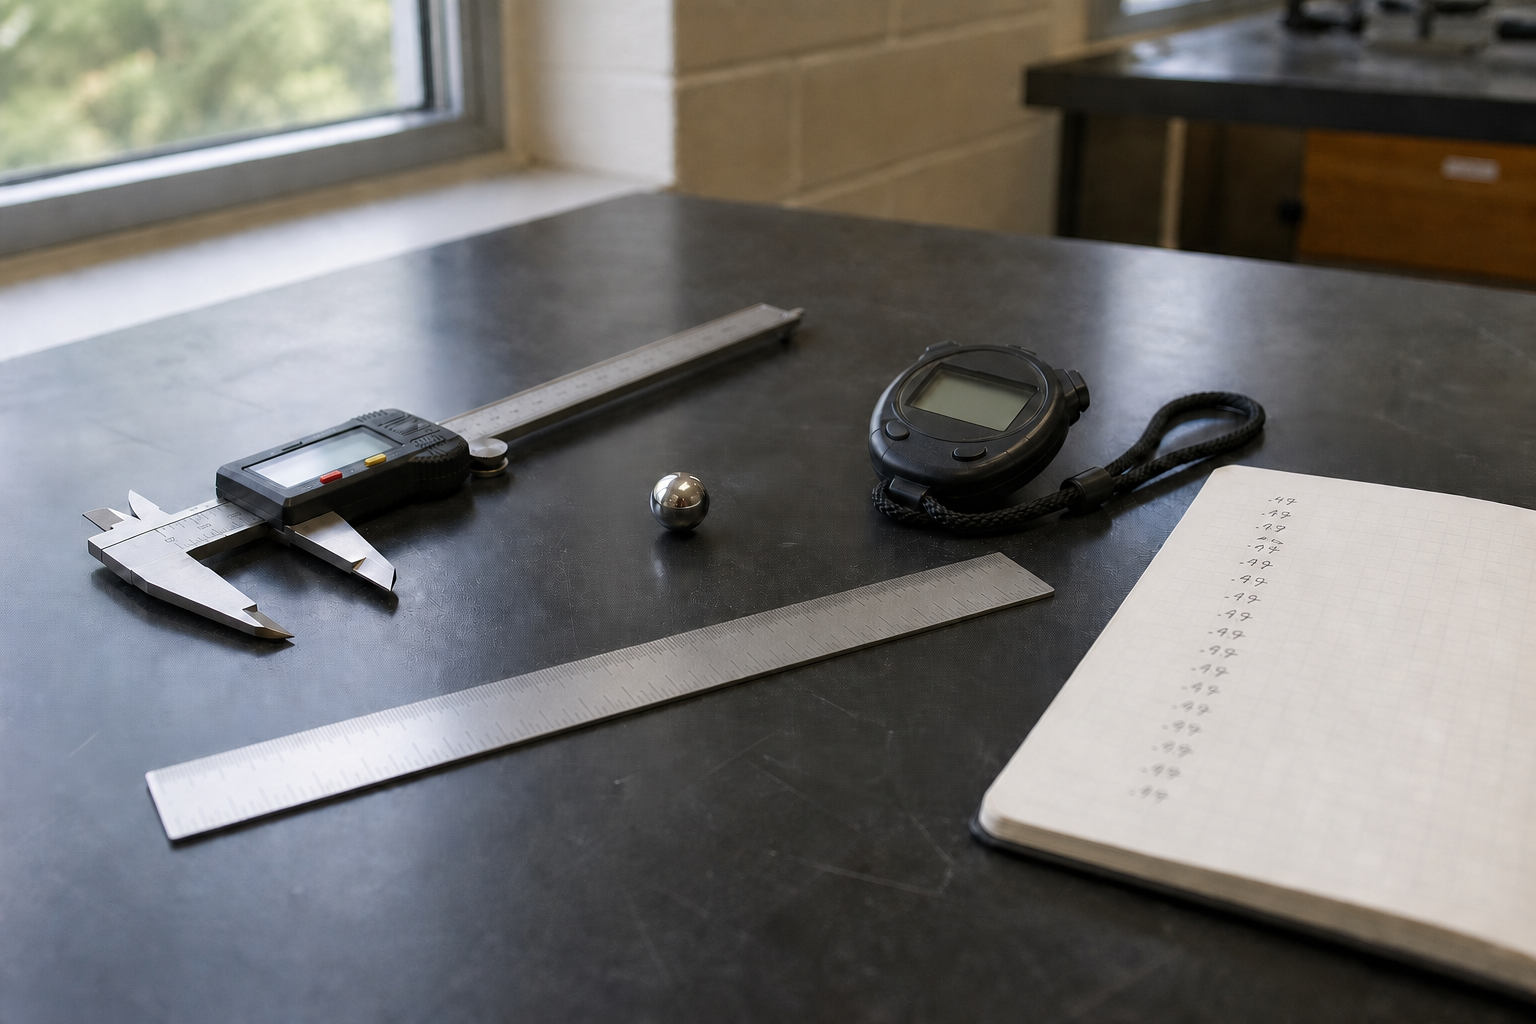
\includegraphics[width=0.60\linewidth]{images/book3/ai/b3-01-lab-bench-measuring.png}

{\small المادة الخام لهذا الفصل: قدمة ذات ورنية، وساعة إيقاف، وكرة، ومسطرة، وعمود من القراءات المكررة التي لا تتفق تمامًا أبدًا.}
\end{omfigure}

\section{مسألة: قياس $g$ بنواس}

\begin{problem}[{مسألة نهاية الأسبوع --- خيط وثقل وساعة إيقاف وشريط
قياس: إلى أي حدّ تستطيع طاولة مطبخ أن تقيس مجال الجاذبية الأرضية،
وأيّ أعدادها الأربعة هو الحلقة الضعيفة}]
\label{pb:b1:units-dimensions:1}
النواس كرة فولاذية معلَّقة من نقطة ثابتة بخيط خفيف؛ ودور التأرجحات
الصغيرة $\tau = 2\pi\sqrt{\ell/g}$ حيث $\ell$ المسافة من نقطة
التعليق إلى مركز الكرة. والهدف الوصول إلى قيمة $g$ بارتياب يمكن الدفاع عنه.

\medskip
\noindent\textbf{الجزء I --- النموذج.}
\begin{enumerate}
  \item تحقق من تجانس $\tau = 2\pi\sqrt{\ell/g}$.
  \item كتلة الكرة $m$. برهن بالأبعاد وحدها على أن الدور لا يمكن أن
        يتوقف على $m$ إذا كان لا يتوقف إلا على $\ell$ و $g$ و $m$.
  \item يتوقف الدور أيضًا، قليلًا، على سعة التأرجح $\theta_0$.
        لماذا يسمح التحليل البعدي بذلك، وماذا يجب فعله تجريبيًّا حتى
        تصير الصيغة قابلة للتطبيق؟
  \item عبّر عن $g$ بدلالة $\ell$ و $\tau$.
\end{enumerate}

\medskip
\noindent\textbf{الجزء II --- قياس الطول.}
شريط القياس مدرَّج بالمليمتر؛ والخيط طوله \qty{99.0}{cm} من التعليق
إلى أعلى الكرة، وقطر الكرة \qty{2.00}{cm}، وقد قُرئ كلٌّ منهما مرة
واحدة.
\begin{enumerate}[resume]
  \item احسب $\ell$.
  \item قيّم الارتياب من النوع B لقراءة واحدة على الشريط.
  \item يضيف تحديدُ نقطة التعليق ومركز الكرة خطأً ممكنًا يُقدَّر
        بمقدار $\pm\qty{5}{mm}$ (توزيع منتظم). ركّبه مع البند
        السابق للحصول على $u(\ell)$، وأعطِ الارتياب النسبي
        $u(\ell)/\ell$.
\end{enumerate}

\medskip
\noindent\textbf{الجزء III --- قياس الدور.}
للتقليل من أثر زمن ردّ الفعل تُوقَّت عشرة أدوار. وثمانية توقيتات من
هذا النوع، بالثانية: $20.12$ و$20.05$ و$20.18$ و$20.09$ و$20.15$
و$20.02$ و$20.11$ و$20.08$.
\begin{enumerate}[resume]
  \item لماذا نوقّت عشرة أدوار لا دورًا واحدًا؟ ولماذا نكرر التوقيت
        ثماني مرات؟
  \item احسب المتوسط $\overline{t_{10}}$ والانحراف المعياري
        التجريبي $s$ للتوقيتات الثمانية.
  \item استنتج \omterm{def:b1:units-dimensions:uncertainty}{الارتياب المعياري} للمتوسط، ثم الدور $\tau$
        وارتيابه $u(\tau)$.
  \item قارن $u(\tau)/\tau$ بالنسبة $u(\ell)/\ell$.
\end{enumerate}

\medskip
\noindent\textbf{الجزء IV --- النتيجة ونقطة ضعفها.}
\begin{enumerate}[resume]
  \item احسب $g$.
  \item اكتب $u(g)/g$ بدلالة $u(\ell)/\ell$ و $u(\tau)/\tau$،
        ثم احسبه.
  \item اكتب النتيجة بالصيغة المعيارية.
  \item قارنها بالقيمة المرجعية $\qty{9.81}{m/s^2}$ عبر \omterm{def:b1:units-dimensions:zscore}{الفارق
        المنسوب}. ما الحكم؟
  \item أيّ المقدارين المقيسين يحدّ من دقة $g$؟ اقترح تحسينين
        ملموسين وقل كم يخفض كلٌّ منهما الارتياب النسبي.
  \item لنفترض أن كل طول قُدّر بزيادة قدرها \qty{5}{mm} بسبب محاذاة
        متسرعة. أهذا محسوب في ميزانية الارتياب؟ وما اسم هذا النوع
        من الخطأ، وكيف يُكشف؟
\end{enumerate}

\medskip
\noindent\textbf{الجزء V --- خمسة أطوال ومستقيم.}
تُعاد التجربة من أجل $\ell = 0.400$ و$0.600$ و$0.800$ و
$1.000$ و\qty{1.200}{m}، فتعطي $\tau^2 = 1.62$ و$2.41$ و$3.25$ و
$4.04$ و\qty{4.84}{s^2}، ولكلٍّ منها $u(\tau^2) \approx 1\%$.
\begin{enumerate}[resume]
  \item لماذا نرسم $\tau^2$ بدلالة $\ell$ لا $\tau$ بدلالة
        $\ell$؟
  \item احسب $\bar\ell$ و $\overline{\tau^2}$.
  \item احسب ميل \omterm{prop:b1:units-dimensions:regression}{المربعات الصغرى} $a$ والمقطع $b$.
  \item استنتج $g$ من الميل.
  \item فسّر المقطع: ماذا يكشف $b$ لو كان غير معدوم بوضوح؟
  \item تعطي الملاءمة الحاسوبية $u(a) = \qty{0.05}{s^2/m}$. استنتج
        $u(g)$ واكتب النتيجة.
  \item قارن نتيجة الطول الواحد في الجزء IV بهذه النتيجة عبر \omterm{def:b1:units-dimensions:zscore}{الفارق
        المنسوب}.
  \item يقترح طالب أن يقيس بدلًا من ذلك تأرجحة واحدة لنواس طوله
        \qty{10}{m} في بئر سلّم، بالشريط وساعة الإيقاف نفسيهما.
        قدّر الارتياب النسبي على $g$ الذي يعطيه ذلك، واستنتج أفضل
        استراتيجية.
\end{enumerate}
\end{problem}
